\documentclass[10pt,]{article}
\usepackage{lmodern}
\usepackage{amssymb,amsmath}
\usepackage{ifxetex,ifluatex}
\usepackage{fixltx2e} % provides \textsubscript
\ifnum 0\ifxetex 1\fi\ifluatex 1\fi=0 % if pdftex
  \usepackage[T1]{fontenc}
  \usepackage[utf8]{inputenc}
\else % if luatex or xelatex
  \ifxetex
    \usepackage{mathspec}
  \else
    \usepackage{fontspec}
  \fi
  \defaultfontfeatures{Ligatures=TeX,Scale=MatchLowercase}
\fi
% use upquote if available, for straight quotes in verbatim environments
\IfFileExists{upquote.sty}{\usepackage{upquote}}{}
% use microtype if available
\IfFileExists{microtype.sty}{%
\usepackage{microtype}
\UseMicrotypeSet[protrusion]{basicmath} % disable protrusion for tt fonts
}{}
\usepackage[left=2cm, right=2cm, top=2cm, bottom=3cm, footskip = .5cm]{geometry}
\usepackage{hyperref}
\hypersetup{unicode=true,
            pdfborder={0 0 0},
            breaklinks=true}
\urlstyle{same}  % don't use monospace font for urls
\usepackage{graphicx,grffile}
\makeatletter
\def\maxwidth{\ifdim\Gin@nat@width>\linewidth\linewidth\else\Gin@nat@width\fi}
\def\maxheight{\ifdim\Gin@nat@height>\textheight\textheight\else\Gin@nat@height\fi}
\makeatother
% Scale images if necessary, so that they will not overflow the page
% margins by default, and it is still possible to overwrite the defaults
% using explicit options in \includegraphics[width, height, ...]{}
\setkeys{Gin}{width=\maxwidth,height=\maxheight,keepaspectratio}
\IfFileExists{parskip.sty}{%
\usepackage{parskip}
}{% else
\setlength{\parindent}{0pt}
\setlength{\parskip}{6pt plus 2pt minus 1pt}
}
\setlength{\emergencystretch}{3em}  % prevent overfull lines
\providecommand{\tightlist}{%
  \setlength{\itemsep}{0pt}\setlength{\parskip}{0pt}}
\setcounter{secnumdepth}{0}

%%% Use protect on footnotes to avoid problems with footnotes in titles
\let\rmarkdownfootnote\footnote%
\def\footnote{\protect\rmarkdownfootnote}

%%% Change title format to be more compact
\usepackage{titling}

% Create subtitle command for use in maketitle
\providecommand{\subtitle}[1]{
  \posttitle{
    \begin{center}\large#1\end{center}
    }
}

\setlength{\droptitle}{-2em}

  \title{}
    \pretitle{\vspace{\droptitle}}
  \posttitle{}
    \author{}
    \preauthor{}\postauthor{}
    \date{}
    \predate{}\postdate{}
  
% Set up the fonts
\usepackage[urw-palatino]{mathdesign}
\usepackage[T1]{fontenc}


% Set the language for 508
\hypersetup{
  pdftitle = {title},
  pdflang = en-US}

% Add accessibility support from http://www.richschwinn.com/accessibility
\RequirePackage{accsupp}
\RequirePackage{pdfcomment}
\newcommand{\AccTool}[2]{\BeginAccSupp{method=pdfstringdef,unicode,Alt={{#1}}}\pdftooltip{{#2}}{{#1}}\EndAccSupp{}}


% Set up the headers and footers
\usepackage{graphicx}
\usepackage{fancyhdr}
\usepackage{ifthen}
\usepackage{everypage}
\usepackage{float}
\usepackage{subfig}

% Avoid struggling over figure and table float in Rmarkdown
\let\origfigure\figure
\let\endorigfigure\endfigure
\renewenvironment{figure}[1][2] {
    \expandafter\origfigure\expandafter[H]
} {
    \endorigfigure
}

\let\origtable\table
\let\endorigtable\endtable
\renewenvironment{table}[1][2] {
    \expandafter\origtable\expandafter[H]
} {
    \endorigtable
}

% First page has the large title and NOAA logo
\pagestyle{fancy}
\fancyhf{}
\setlength\headheight{40pt}
\cfoot{\thepage}

\AddEverypageHook{%
   \ifthenelse{\value{page}=1}%
     {\rhead{
\includegraphics[width=40pt]{images/NOAA_logo.png} \\ \textsf{\emph{Published March 20, 2019}}}
      \lhead{\textsf{\LARGE State of the Ecosystem 2019: Mid-Atlantic}}
      }%
     {\rhead{}
      \lhead{\textsf{\emph{State of the Ecosystem 2019: Mid-Atlantic}}}
     }
}

\renewcommand{\headrulewidth}{0.4pt}
\renewcommand{\footrulewidth}{0pt}

% Make caption fonts a bit smaller
\usepackage[font={small}]{caption}


% Change section labels to san serif
\usepackage{sectsty}
\allsectionsfont{\normalfont\sffamily\bfseries}
\usepackage{booktabs}
\usepackage{longtable}
\usepackage{array}
\usepackage{multirow}
\usepackage{wrapfig}
\usepackage{float}
\usepackage{colortbl}
\usepackage{pdflscape}
\usepackage{tabu}
\usepackage{threeparttable}
\usepackage{threeparttablex}
\usepackage[normalem]{ulem}
\usepackage{makecell}
\usepackage{xcolor}

\begin{document}

\section{Overview}\label{overview}

The purpose of this report is to synthesize available information
relevant to fishery management in the Mid-Atlantic portion of the US
Northeast Shelf. This 2019 report highlights where management
interventions have proven successful to achieve ecological objectives,
but also characterizes the considerable challenges for management posed
by climate change and increasing trade-offs across conservation,
fishing, and other human activities in this region (Fig.
\ref{fig:conceptual-model}). Finally, we describe combinations of
ecological signals that present opportunities for further integrated
research and possibly creative management solutions.

\begin{figure}

{\centering 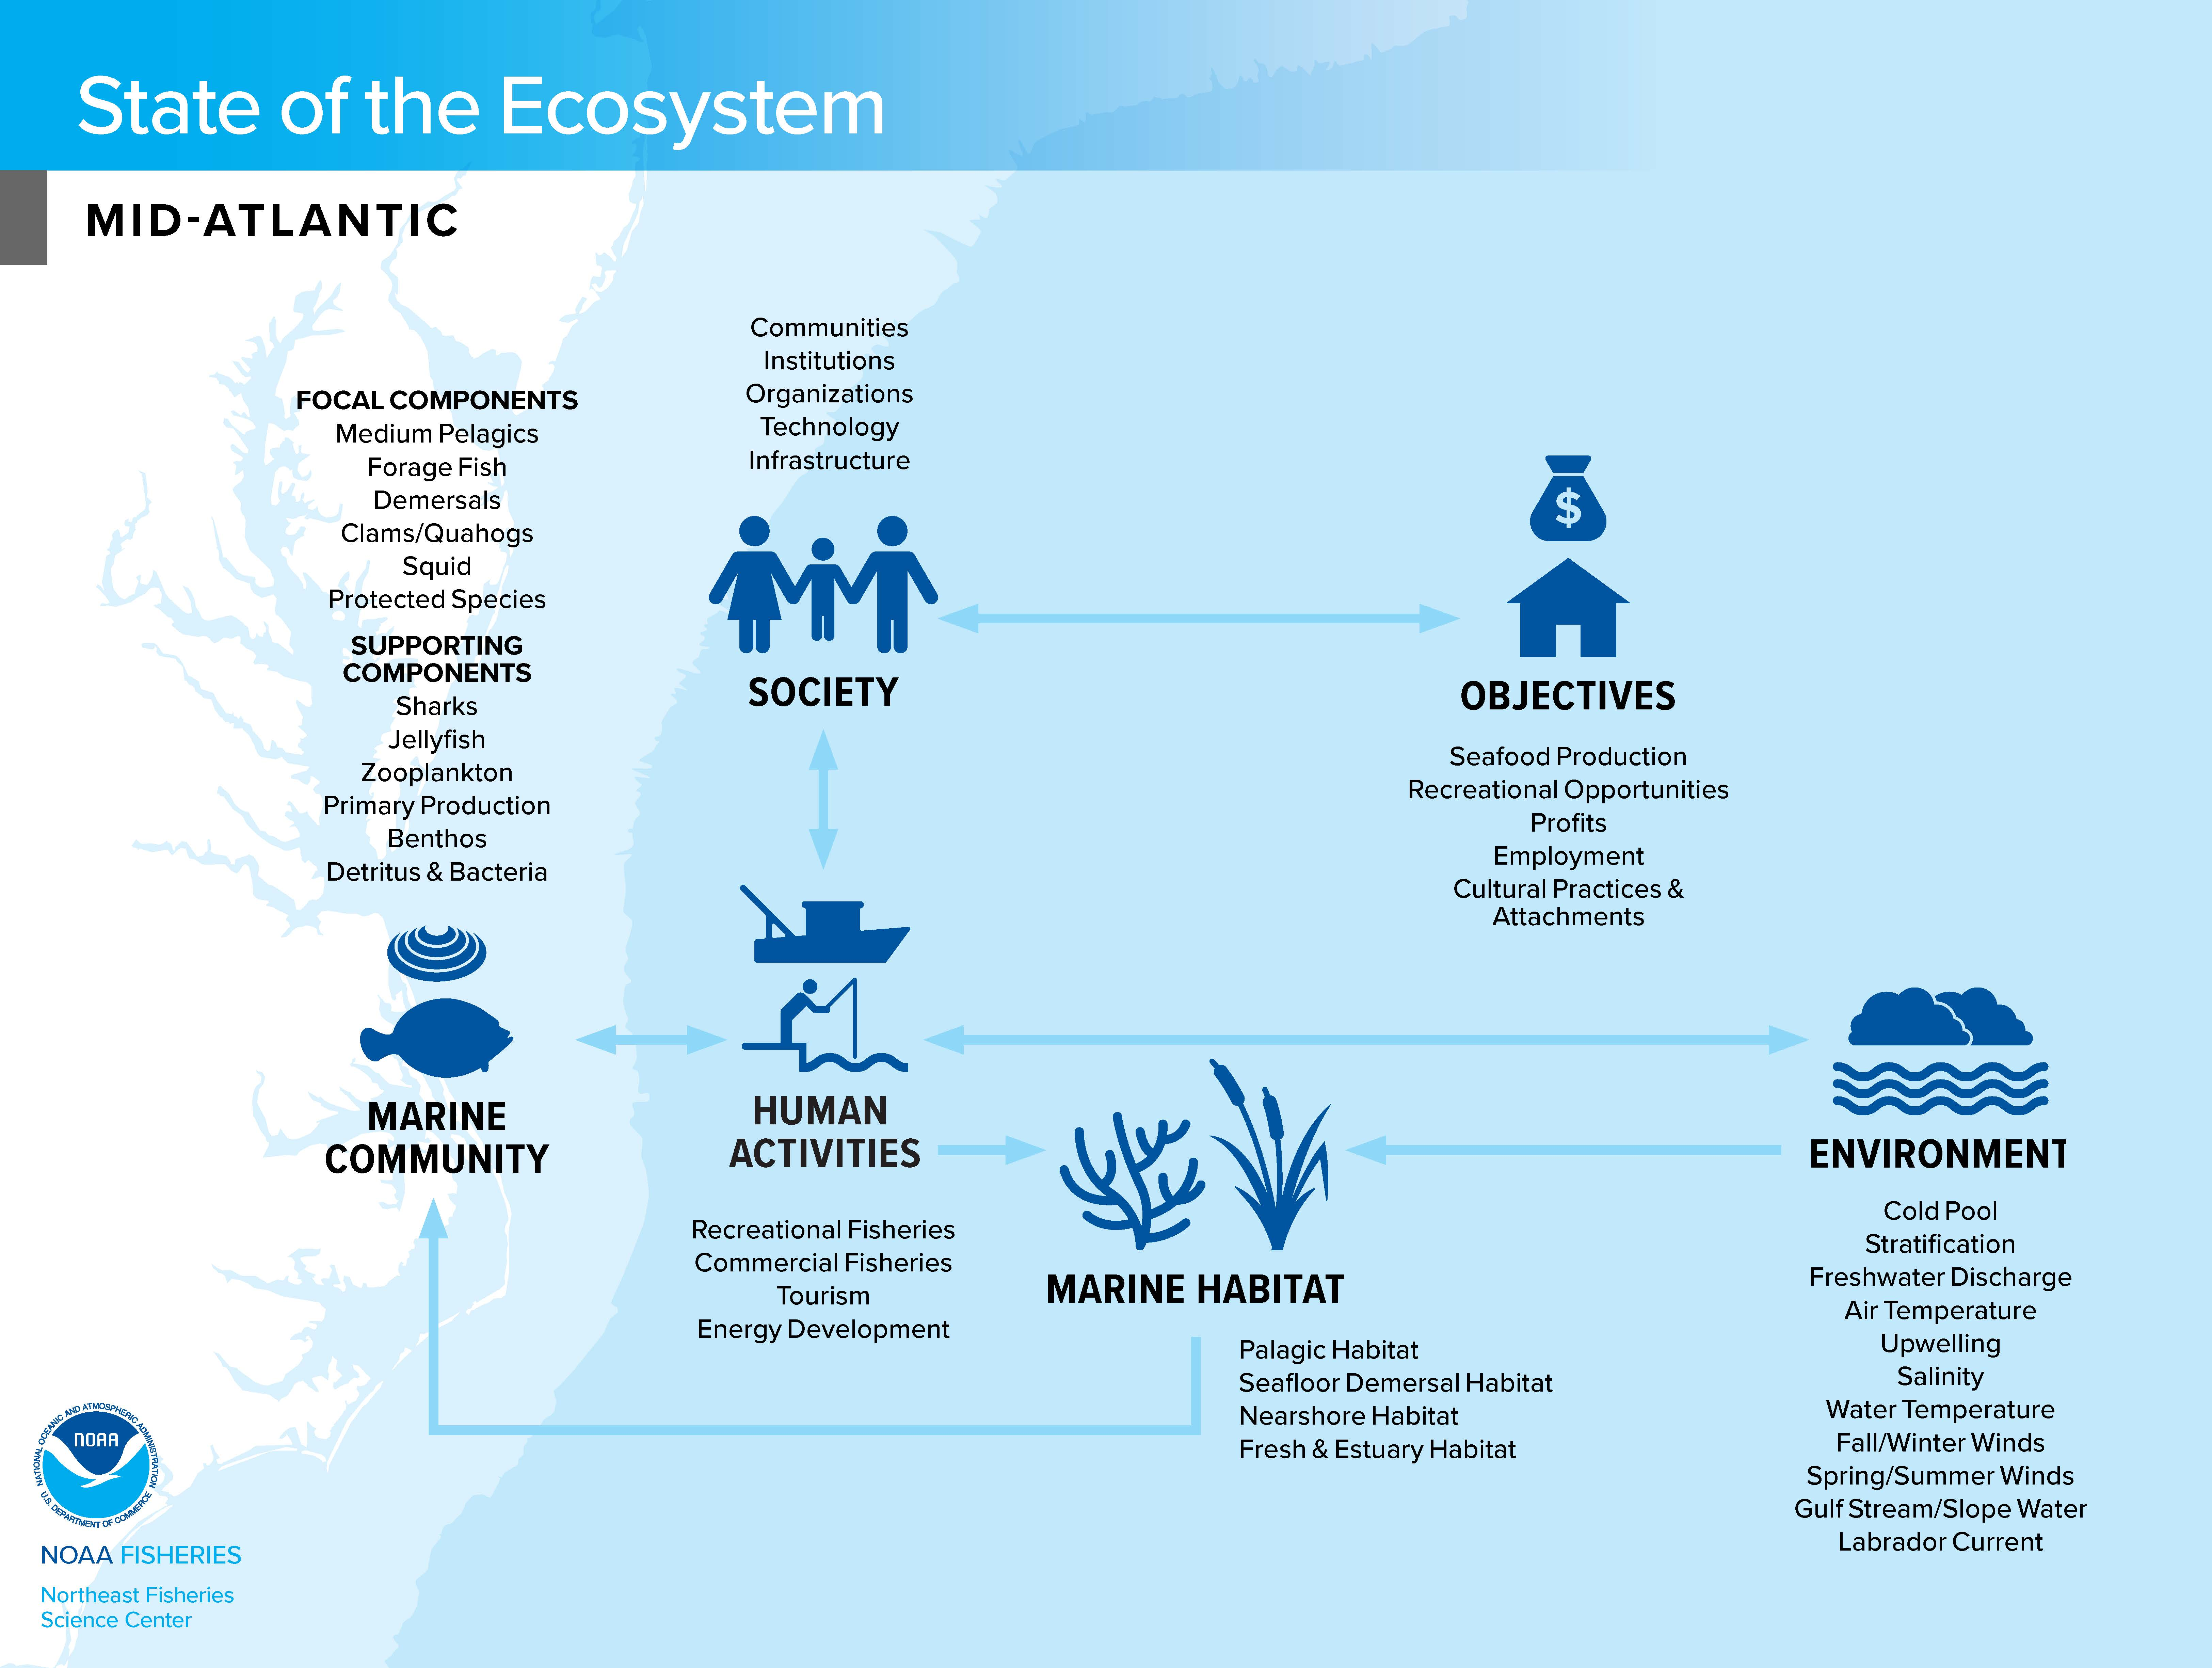
\includegraphics[width=\textwidth]{images/MAB_conmod_overview} 

}

\caption{A conceptual model places detailed species-level management in context by highlighting relationships between focal species groups organized by the Mid-Atlantic Fisheries Management Council (MAFMC) Fishery Management Plan (FMP), managed human activities, environmental drivers, habitats, and key ecological links.}\label{fig:conceptual-model}
\end{figure}

Some management interventions for ecosystems and fisheries have proven
beneficial in the Mid-Atlantic and throughout the Northeast US Shelf.
For example, the evidence suggests that management limiting nutrient
inputs has significantly improved water quality in Chesapeake Bay (Fig.
\ref{fig:cb-attainment}). This trend, which has been driven by
improvements to dissolved oxygen content and water clarity, has positive
implications for aquaculture development and for managed species using
the Bay as nursery habitat. Also encouraging is a continued decrease in
harbor porpoise bycatch, which for this year is the lowest on record in
the Northeast US, and an apparent stable harbor porpoise population
(Fig. \ref{fig:harbor-porpoise-bars}).

However, there are multiple signals indicating challenges to meeting
management goals. Despite mostly meeting fishery management objectives
at the single species level (Fig. \ref{fig:stock-status}), long term
declines in total seafood production and commercial revenue remain
apparent (Figs. \ref{fig:total-landings}, \ref{fig:comm-landings},
\ref{fig:comm-revenue}). Indicators highlight a declining diversity of
recreational opportunities (fishing modes and species, Fig.
\ref{fig:rec-div}). Further, coastal communities with high fishery
engagement and reliance are dependent on a smaller number of species
than historically. These species are predominantly high valued shellfish
vulnerable to increased ocean temperature and acidification.

Fisheries are significantly affecting protected species, particularly
large whale abundance. Changes in fishery management to address this
issue could have considerable consequences for the fixed gear fishing
sector, particularly for pot gear. The recovery of North Atlantic right
whales is affected by anthropogenic mortality (Fig.
\ref{fig:NARW-abundance}). Shifts in ecosystem conditions may be
contributing to increased interaction between right whales and fishing
gear and could be playing a role in other protected species trends.
Unusual Mortality Events (UMEs) have been declared for North Atlantic
right whales, humpback whales, and minke whales, and preliminary
investigations suggest fishing gear entanglement has played a primary
role in these mortalities. Gray seal bycatch mortality has also risen in
recent years, with an estimated annual mortality that has often totaled
more than 1000 animals and a UME has been declared for both gray and
harbor seals that may be due to phocine distemper virus.

Several climate and ecosystem observations are trending towards
unprecedented levels. The Northeast US shelf is still among the fastest
warming waters globally (Fig. \ref{fig:long-term-sst}) with implications
for species physiology, productivity, distribution, and community
composition. Globally, 2018 was the 4th warmest year on record with the
last four years being the warmest on record. In the Mid-Atlantic, 2018
summer sea surface temperatures were the third highest on record, while
temperatures during the other seasons were near or slightly below
average (Fig. \ref{fig:MAB-SST-insitu}). Annual average bottom
temperature measurements show a significant long term warming trend
(Fig. \ref{fig:MAB-bot-temp}). Ocean circulation is changing as well.
The position of the northern edge of the Gulf Stream has trended
northward since the late 1950s, with an increasing rate since 2009. The
most northerly positions on record were observed between 2014-2017 (Fig.
\ref{fig:GSI}). A more northerly Gulf Stream position is generally
associated with warmer ocean temperature in the Northeast US shelf
{[}\protect\hyperlink{ref-zhang_role_2007}{1}{]} and increased sea
surface height along the U.S. east coast
{[}\protect\hyperlink{ref-goddard_extreme_2015}{2}{]}.

The management implications of these ocean changes vary by region and
species, and are not fully understood at this point. Changes in the
distribution of managed fish species continue, with aggregate trends on
the entire Northeast Shelf shifting towards the northeast and generally
into deeper water (Fig. \ref{fig:spec-dist}). These shifts place
increasing pressure on the management system. The proportion of NEFMC
(New England Fishery Management Council) managed benthivore species
(righteye flounders, haddock) has declined over time in Mid-Atlantic
waters according to bottom trawl surveys (Fig. \ref{fig:NEFMC-in-MAB}),
while the proportion of MAFMC (Mid-Atlantic Fishery Management Council)
managed planktivore (squids, mackerel, and butterfish) species has been
increasing in New England waters in both surveys and landings (Figs.
\ref{fig:MAFMC-in-NE}, \ref{fig:comm-landings}). Similarly, butterfish
have been observed in Gulf of Maine common tern fledgling diets between
2009-2011 and again in 2018 (see New England report). The downward trend
in recreational species diversity in the Mid-Atlantic (Fig.
\ref{fig:rec-div}) contrasts with an increase in recreational species
diversity over time in New England (see New England report), although it
is unclear to what extent this result is due to the aggregation of SAFMC
species in the indicator itself. Nearshore NEAMAP survey indices show
some similar patterns to offshore surveys, although with different
magnitudes, perhaps reflecting seasonal importance of nearshore habitats
(Fig. \ref{fig:nefsc-biomass-mab}); these patterns will be explored in
more detail in future analyses. As temperature and ocean circulation
indicators trend toward extremes, fishery management based on static
stock areas will likely face continued changes in species distribution.

Observed changes at the base of the food web, including timing and
community composition, affect productivity of protected and managed
species in ways we do not yet fully understand. There is a trend of
increasing primary production in the Mid-Atlantic, but this trend is
primarily driven by increased summer production, which is due to warmer
temperatures and increased bacterial remineralization and nutrient
recycling (Fig. \ref{fig:PP-OCCI}). This increased productivity is most
likely from smaller-celled species that contribute less to fish
production compared to larger phytoplankton. Current zooplankton trends
in the Mid-Atlantic suggest a shift in timing towards a spring peak in
the dominant species (Fig. \ref{fig:MAB-oi-zoo}), as well as a shift
towards smaller-bodied copepods (Fig. \ref{fig:MAB-sli}). This suggests
a possible return to conditions last observed during the 1990s, when
small bodied copepods dominated the zooplankton community, regime shifts
in groundfish recruitment were observed
{[}\protect\hyperlink{ref-perretti_regime_2017}{3}{]}, and North
Atlantic right whales experienced lower birth rates
{[}\protect\hyperlink{ref-greene_remote_2013}{4}{]}. The timing of
shifts in fish condition may be similar (Fig. \ref{fig:mab-cf}), though
potential mechanisms connecting adult fish condition to zooplankton
patterns require further study.

\section{Report Structure}\label{report-structure}

The major messages of the report are synthesized above with reference to
key figures. The information in this report is organized around general
ecosystem-level management objectives (Table
\ref{tab:management-objectives}), and indicators related to these
objectives are grouped into four general categories in the four sections
below: economic and social, protected species, fish and invertebrates,
and habitat quality and ecosystem productivity. Each section begins with
a summary of main messages with links to other sections, including any
new information added at the request of the Fishery Management Councils,
and includes figures with brief descriptions of all current indicators.
Detailed technical methods documentation\footnote{\url{https://NOAA-EDAB.github.io/tech-doc}}
and indicator data\footnote{\url{https://github.com/NOAA-EDAB/ecodata}}
are available online. The details of standard figure formatting (Fig.
\ref{fig:docformat}a), categorization of fish and invertebrate species
into feeding groups (Table \ref{tab:species-groupings}), and definitions
of ecological production units (EPUs, including the Mid-Atlantic Bight,
MAB; Fig. \ref{fig:docformat}b) are provided at the end of the document.

\begin{table}[!h]

\caption{\label{tab:management-objectives}Established ecosystem-scale objectives in the Mid-Atlantic Bight}
\centering
\begin{tabular}{ll}
\toprule
\textbf{Objective Categories} & \textbf{Indicators reported here}\\
\midrule
Seafood Production & Landings by feeding guild\\
Profits & Revenue by feeding guild\\
Recreation & Number of anglers and trips; recreational catch\\
Stability & Diversity indices (fishery and species)\\
Social \& Cultural & Commercial and recreational reliance\\
\addlinespace
Biomass & Biomass or abundance by feeding guild from surveys\\
Productivity & Condition and recruitment of MAFMC managed species\\
Trophic structure & Relative biomass of feeding guilds, primary productivity\\
Habitat & Estuarine and offshore habitat conditions\\
\bottomrule
\end{tabular}
\end{table}

\section{Economic and Social}\label{economic-and-social}

The objectives of U.S. federal fishery management include providing
benefits to the Nation in terms of seafood production and recreational
opportunities, while considering economic efficiency and effects on
coastal communities. The indicators in this section consider these
objectives for commercial and recreational fishing sectors separately
where possible.

Despite mostly meeting fishery management objectives at the single
species level (Fig. \ref{fig:stock-status}), long term declines in total
seafood production and commercial revenue remain apparent. Indicators
highlight a declining diversity of recreational opportunities (fishing
modes and species). Further, coastal communities with high fishery
engagement and reliance are dependent on a smaller number of species
than historically, these species are predominantly high valued shellfish
vulnerable to increased ocean temperature and acidification.

\subsection{Commercial sector (MAB)}\label{commercial-sector-mab}

Seafood landings overall and for MAFMC managed species are declining
(Fig. \ref{fig:total-landings}). Seafood landings for feeding guilds are
also stable or declining (Fig. \ref{fig:comm-landings}), with the
exception of a long term increase in MAFMC managed benthivores (scup,
black sea bass, and tilefish). In 2018, landings of MAFMC managed
planktivores increased to account for nearly all planktivore landings in
the MAB, likely due to increased squid and decreased Atlantic herring
landings.

\begin{figure}

{\centering \includegraphics{SOE-MAFMC-2019_files/figure-latex/total-landings-1} 

}

\caption{Total commercial seafood landings (black) and Mid-Atlantic managed seafood landings (red).}\label{fig:total-landings}
\end{figure}

\begin{figure}

{\centering \includegraphics{SOE-MAFMC-2019_files/figure-latex/comm-landings-1} 

}

\caption{MAFMC managed species landings (red) and total commercial landings (black) by feeding guild.}\label{fig:comm-landings}
\end{figure}

Revenue for MAFMC managed species has also declined over the long term
(Fig. \ref{fig:comm-revenue}), with recent decreases in total revenue
driven by decreased landings volume outweighing increased prices for
benthos, planktivores, and other species groups (Fig. \ref{fig:bennet}).

\begin{figure}

{\centering \includegraphics{SOE-MAFMC-2019_files/figure-latex/comm-revenue-1} 

}

\caption{Total revenue for the region (black) and revenue from MAFMC managed species (red).}\label{fig:comm-revenue}
\end{figure}

\begin{figure}

{\centering \includegraphics{SOE-MAFMC-2019_files/figure-latex/bennet-1} 

}

\caption{Revenue change from the long-term mean in 2015 dollars (black), Price (PI), and Volume Indicators (VI) for commercial landings in the Mid-Atlantic.}\label{fig:bennet}
\end{figure}

MAB fishing communities are heavily reliant on shellfish species
(especially scallops) for the majority of revenue. This reliance likely
represents heightened risk to fishing communities, particularly along
the coasts of New York, New Jersey, and Virginia in ports which are
highly engaged and reliant on commercial fishing. This risk is
heightened by the high climate vulnerability of shellfish to ocean
acidification (Fig. \ref{fig:MAB-comm-reliance-maps-outlined}).

\begin{figure}

{\centering \includegraphics{SOE-MAFMC-2019_files/figure-latex/MAB-comm-reliance-maps-outlined-1} 

}

\caption{Commercial engagement (total pounds landed, value landed, commercial permits and commercial dealers in a community) and reliance (per capita engagement) based on 2016 landings and the ACS running average of 2012-2016 census data.}\label{fig:MAB-comm-reliance-maps-outlined}
\end{figure}

Aquaculture production in the Mid-Atlantic is dominated by shellfish as
well. Virginia continues to lead oyster production in the US, though
numbers sold stabilized in 2017 after a long term increase. Reported
concerns for Virginia growers within the past two years include an
increase in wild spat fall preventing farmed oysters from entering
higher-value markets. Maryland and New Jersey oyster production
continues to increase (Fig. \ref{fig:oyster-aqua}).

\begin{figure}

{\centering \includegraphics{SOE-MAFMC-2019_files/figure-latex/oyster-aqua-1} 

}

\caption{Oyster aquaculture production in terms of number of oysters sold from Virginia, Maryland, and New Jersey.}\label{fig:oyster-aqua}
\end{figure}

Commercial fleet diversity indices were updated with 2017 data. Current
diversity remains near the long term average.

\subsection{Recreational sector (Mid-Atlantic
states)}\label{recreational-sector-mid-atlantic-states}

All recreational indicators have been updated with new Marine
Recreational Information Program (MRIP) data, and new indicators for
recreational diversity are presented in this report at the request of
the MAFMC. In contrast to the commercial seafood production trends,
recreational seafood production shows an increasing trend since the
mid-1990s with the updated MRIP data (Fig. \ref{fig:rec-landings}))

\begin{figure}

{\centering \includegraphics{SOE-MAFMC-2019_files/figure-latex/rec-landings-1} 

}

\caption{Total recreational seafood harvest in the Mid-Atlantic region.}\label{fig:rec-landings}
\end{figure}

Updated indicators for recreational opportunities (effort days and
number of anglers) show general increases since the 1990s, peaking in
the late 2000s and declining since then. This is similar to previously
reported trends (Fig. \ref{fig:rec-op}).

\begin{figure}

{\centering \includegraphics{SOE-MAFMC-2019_files/figure-latex/rec-op-1} 

}

\caption{Recreational effort and number of recreational anglers in the Mid-Atlantic.}\label{fig:rec-op}
\end{figure}

Newly developed indicators for the diversity of recreational effort
(i.e.~access to recreational opportunities) by mode (party/charter
boats, private boats, shore-based), and diversity of catch (NEFMC and
MAFMC managed species only) show significant long-term downward trends.
The downward effort diversity trend is driven by party/charter
contraction (from a high of 24\% of angler trips to 6\% currently), with
a shift towards shorebased angling. Effort in private boats remained
stable between 36-37\% of angler trips across the entire series. The
long-term decrease in catch diversity in the Mid-Atlantic states
contrasts with an increase in recreational catch diversity in New
England states over the same time period; this trend requires further
investigation as SAFMC managed species are not currently tracked
separately (Fig. \ref{fig:rec-div})

\begin{figure}

{\centering \includegraphics{SOE-MAFMC-2019_files/figure-latex/rec-div-1} 

}

\caption{Recreational effort diversity and diversity of recreational catch in the Mid-Atlantic.}\label{fig:rec-div}
\end{figure}

Recreational fishing is important to many Mid-Atlantic communities,
particularly on Long Island, the New Jersey shoreline and the Delaware
Bay. Communities that are most socially and economically dependent (both
engaged and reliant) on recreational fishing may face additional risk
due this downward shift in diversity of recreational opportunity and
species catch (Fig. \ref{fig:MAB-rec-engage}).

\begin{figure}

{\centering \includegraphics{SOE-MAFMC-2019_files/figure-latex/MAB-rec-engage-1} 

}

\caption{Recreational engagement (shore, private vessel and for-hire recreational fishing in a community) and reliance (per capita engagement) based on 2016 landings and the ACS running average of 2012-2016 census data.}\label{fig:MAB-rec-engage}
\end{figure}

\newpage

\section{Protected Species}\label{protected-species}

Protected species include marine mammals (under the Marine Mammal
Protection Act), endangered and threatened species (under the Endangered
Species Act), and migratory birds (under the Migratory Bird Treaty Act).
In the Northeast US, endangered/threatened species include Atlantic
salmon, Atlantic and shortnose sturgeon, all sea turtle species, and 5
baleen whales. Fishery management objectives for protected species
generally focus on reducing threats and on habitat
conservation/restoration; here we report on the status of these actions
as well as indicating the potential for future interactions driven by
observed and predicted ecosystem changes in the Northeast US region.
This year four Unusual Mortality Events (UMEs) have been declared for
three large whale species and two seal species, with several mortalities
attributed to human interactions. Also, a marine mammal climate
vulnerability assessment is currently underway for Atlantic and Gulf of
Mexico populations and will be reported on in future versions of this
report. Strong evidence exists to suggest that the level of interaction
between right whales and the combination of fixed gear in the US and
Canada is contributing substantially to the decline of the species.

\subsection{Sea turtles (coastwide)}\label{sea-turtles-coastwide}

Sea turtles are known to be susceptible to climate and ecosystem
changes, and their distribution is influenced by water temperature. Sea
turtle diets contain a considerable amount of gelatinous zooplankton,
which are also influenced by changes in the ecosystem. At present,
management measures to reduce sea turtle-fishery interactions are
limited to the regions with historical observations of sea turtles and
based on historical ocean temperature distributions. However, changes in
climate may cause turtles to shift northward into areas with heavy
fishing, possibly resulting in increased bycatch.

\subsection{Whales (coastwide)}\label{whales-coastwide}

North Atlantic right whales are among the most endangered large whale
populations in the world. Changes in right whale trends can have
implications for fisheries management where fisheries interact with
these whales. Additional management restrictions could have a large
impact on fishing times, gears, etc. Although the population increased
steadily from 1990 to 2011, it has decreased recently (Fig.
\ref{fig:NARW-abundance}). From
{[}\protect\hyperlink{ref-pace_statespace_2017}{5}{]}: ``The probability
that the population's trajectory post-2010 was a decline was estimated
at 99.99\%.'' Reduced survival rates of adult females and diverging
abundance trends between sexes have also been observed. It is estimated
that there are only about 100 adult females remaining in the population.
Further, right whale distribution has changed since 2010. The reasons
for these changes is unclear, but changes in climate and primary prey
(\emph{Calanus finmarchicus}) are suspected.

Three large whale Unusual Mortality Events (UMEs) have been declared for
North Atlantic right whales, humpback whales, and minke whales. In all
three cases human interaction appears to have contributed to increased
mortalities, although investigations are not complete. Twenty right
whale mortalities have been documented in 2017 and 2018 so far. Among
the 20 right whale deaths observed in 2017 and 2018 thus far, 5 were due
to vessel strike (1 in US waters, 4 in Canadian waters), 6 from
entanglement (2 in Canadian gear, 1 in unknown gear, and 3 others found
in US waters), and the rest from unknown causes. UMEs have also been
declared for humpback whales during 2016-2018 and 2017-2018 minke whales
due to elevated strandings. Necropsy investigations on 50\% of humpback
whales showed evidence of human interaction, either ship strike or
entanglement. Similarly, 60\% of minke whales show evidence of human
interactions or infectious disease. In both cases the investigations are
still underway and more research is needed to determine the causes of
these UME.

\begin{figure}

{\centering \includegraphics{SOE-MAFMC-2019_files/figure-latex/NARW-abundance-1} 

}

\caption{Right whale abundance estimates with 95\% credible intervals. These values represent the estimated number of animals alive sometime during the year referenced and NOT at the end of the year referenced. Seventeen known deaths were recorded in 2017 (likely all from anthropogenic causes), but these deaths were not reflected in the 2017 estimate because those animals were alive sometime during the year.}\label{fig:NARW-abundance}
\end{figure}

\subsection{Grey seals (coastwide)}\label{grey-seals-coastwide}

The number of grey seals (\emph{Halichoerus grypus}) in U.S. waters has
risen dramatically in the last 2 decades, with few observed in the early
1990s to roughly 24,000 observed in southeastern Massachusetts in 2015
(Pace et al. in press). Roughly 30,000 - 40,000 gray seals were
estimated in southeastern Massachusetts in 2015, using correction
factors applied to seal counts visible in Google Earth imagery. As of
2016, the size of the grey seal population in Canada, which is part of
the same stock as the grey seals in the U.S., was estimated to be
roughly 425,000, and increasing by 4\% a year. Pups born on Muskeget
Island MA, currently the largest pupping site for gray seals in the
U.S., were first observed in 1988 and now number over 3,500. Trends in
pup production at U.S. colonies appear to be increasing, and it is
likely that U.S. pup production is being supplemented each year by
animals from Canada. A UME for both gray and harbor seals was declared
in 2018, triggering an investigation into the cause of this event. Tests
so far suggest phocine distemper virus as a potential cause, although
the investigation is not yet complete.

Fisheries interactions have increased over the past 2 decades, with
fewer than 10 total estimated grey seal interactions in 1993, to more
than 1000 in 2013 and 2015, and with preliminary 2017 estimates over
900. Analysis of seal diet is currently underway using a variety of
techniques (analysis of stomach contents, fatty acids, and DNA) to
assess the potential impact of seal population growth on the ecosystem
and important commercial fish species.

\subsection{Harbor porpoise
(coastwide)}\label{harbor-porpoise-coastwide}

Harbor porpoise bycatch has resulted in fisheries closures in the past,
but current bycatch levels suggest that management measures have been
effective, reducing this fishery interaction. The 5-year mean bycatch
has been below the maximum permitted level (Potential Biological
Removal, PBR) since 2011 (Fig. \ref{fig:harbor-porpoise-bars}), and the
2016 and draft 2017 annual bycatch estimates are among the lowest in the
time series. Recent compliance with the harbor porpoise take reduction
plan and reduced fishing effort are thought to contribute to low bycatch
estimates. Potential recent shifts in porpoise distribution could also
be contributing to low bycatch and this will be explored during the
coming year. A new draft harbor porpoise abundance estimate suggests
stable or increasing abundance of the Gulf of Maine/Bay of Fundy harbor
porpoise stock. Recent analyses have examined regional harbor porpoise
diet, and suggest that harbor porpoise are not typically feeding on fish
caught in gillnets. However, the impact of ecosystem changes on bycatch,
population, or distribution remain unclear.

\begin{figure}

{\centering \includegraphics{SOE-MAFMC-2019_files/figure-latex/harbor-porpoise-bars-1} 

}

\caption{Harbor porpoise bycatch estimate (black) shown with Potential Biological Removal (red). Error bars indicate 95\% confidence interval.}\label{fig:harbor-porpoise-bars}
\end{figure}

\subsection{Protected Fish (coastwide)}\label{protected-fish-coastwide}

Shortnose sturgeon (endangered) and five distinct populations segments
(DPS) of Atlantic sturgeon are found in coastal waters of the
mid-Atlantic (endangered: New York Bight, Chesapeake Bay, Carolina, and
South Atlantic; threatened: Gulf of Maine). Multiple populations spawn
in mid-Atlantic watersheds and river-ocean connectivity is an important
habitat characteristic. These populations are vulnerable to climate and
ecosystem changes as their life history results in high biological
sensitivity and habitat needs result in very high climate exposure.
Threat reductions are focused on protecting critical habitat, habitat
restoration, reducing ship-strikes, and bycatch reduction. Endangered
Gulf of Maine Atlantic salmon are rarely found this far south but fish
from the Connecticut River legacy program may be found in coastal waters
of this area.

\newpage

\section{Fish and Invertebrates}\label{fish-and-invertebrates}

Fishery management aims to keep individual harvested species within
population ranges where productivity is maximized over the long-term.
However, these managed species represent a subset of the full ecosystem,
interacting with a wider range of predators and prey and relying on
diverse habitats. Indicators in this section summarize single species
status as well as tracking trends for broad categories of fish within
the ecosystem, including changes in biomass, distribution, condition,
and diversity. Changes in overall predator and prey levels as well as
distribution have implications for managed fish productivity, fishing
operations, and regional fishery management.

\subsection{Stock status and aggregate distribution
(coastwide)}\label{stock-status-and-aggregate-distribution-coastwide}

Single species management objectives of maintaining biomass above
minimum thresholds and fishing mortality below limits are being met for
all but one MAFMC managed species, though the status of four stocks is
unknown (Fig. \ref{fig:stock-status}).

\begin{figure}

{\centering \includegraphics{SOE-MAFMC-2019_files/figure-latex/stock-status-1} 

}

\caption{Summary of single species status for MAFMC and jointly managed stocks.}\label{fig:stock-status}
\end{figure}

Changes in the distribution of managed fish species continue, with
aggregate trends on the entire Northeast Shelf towards the northeast and
generally into deeper water (Fig. \ref{fig:spec-dist}). These shifts
will place increasing pressure on the management system.

\begin{figure}

{\centering \includegraphics{SOE-MAFMC-2019_files/figure-latex/spec-dist-1} 

}

\caption{Aggregate species distribution metrics for species in the Northeast Large Marine Ecosystem.}\label{fig:spec-dist}
\end{figure}

\subsection{Survey biomass (MAB)}\label{survey-biomass-mab}

As in past years, piscivore trends differ by season, with a significant
long term decline in fall and an increase in spring (Fig.
\ref{fig:nefsc-biomass-mab}). However, nearshore survey indices
(Northeast Area Monitoring and Assessment Program; NEAMAP) suggest a
decline for piscivores in spring. Surveys in both seasons may be
sampling different groups of dominant species; for example the
divergence in spring piscivores between offshore and NEAMAP surveys may
represent the difference in inshore versus offshore distribution of
spiny dogfish. Overall the NEAMAP surveys show similar patterns to
offshore surveys for planktivores and benthivores, although with
different magnitudes, perhaps reflecting seasonal importance of
nearshore habitats. These patterns will be explored in more detail in
future analyses.

\begin{figure}

{\centering \includegraphics{SOE-MAFMC-2019_files/figure-latex/nefsc-biomass-mab-1} 

}

\caption{Fall (left) and spring (right) surveyed biomass in the Mid-Atlantic Bight. Data from the NEFSC Bottom Trawl Survey are shown in black, with NEAMAP shown in red.}\label{fig:nefsc-biomass-mab}
\end{figure}

The proportion of NEFMC managed benthivore species (righteye flounders,
haddock) has declined over time in Mid-Atlantic waters according to
bottom trawl surveys (Fig. \ref{fig:NEFMC-in-MAB}), while the proportion
of MAFMC managed planktivore (squids, mackerel and butterfish) species
has been increasing in New England waters in both surveys and landings
(Fig. \ref{fig:MAFMC-in-NE}, Fig. \ref{fig:comm-landings}).

\begin{figure}

{\centering \includegraphics{SOE-MAFMC-2019_files/figure-latex/NEFMC-in-MAB-1} 

}

\caption{New England-managed survey proportion of MAB benthivores.}\label{fig:NEFMC-in-MAB}
\end{figure}

\begin{figure}

{\centering \includegraphics{SOE-MAFMC-2019_files/figure-latex/MAFMC-in-NE-1} 

}

\caption{Mid-Atlantic-managed survey proportion of GOM and GB planktivores.}\label{fig:MAFMC-in-NE}
\end{figure}

Other observations corroborate these survey trends. For example,
butterfish have been observed in Gulf of Maine common tern fledgling
diets between 2009-2011 and again in 2018 (see New England report). The
downward trend in recreational species diversity in the Mid-Atlantic
(Fig. \ref{fig:rec-div}) contrasts with an increase in recreational
species diversity over time in New England (see New England report),
although it is unclear to what extent this result is due to the
aggregation of SAFMC species in the indicator itself. As temperature and
ocean circulation indicators trend toward extremes (next section),
fishery management will likely face continued changes in species
distribution.

\subsection{Fish condition (coastwide, MAFMC managed
stocks)}\label{fish-condition-coastwide-mafmc-managed-stocks}

Fish condition is measured as the weight at a given length in relation
to the average - a measure of `fatness' and a factor that influences
fecundity. This information is from fall NEFSC bottom trawl surveys.
Overall, condition factor has been mixed for the past decade, in
contrast to overall high condition up to 2000 and overall lower
condition for 2001-2010 (Fig. \ref{fig:mab-cf}). The timing of these
shifts is similar to shifts in the small-large zooplankton indicator
(Fig. \ref{fig:MAB-sli}). Condition factor for some MAFMC managed
predators (bluefish, spiny dogfish) was high in 2018. Black sea bass
condition was low in 2018. 2017 information is missing for some species
due to the incomplete 2017 fall survey.

\begin{figure}

{\centering 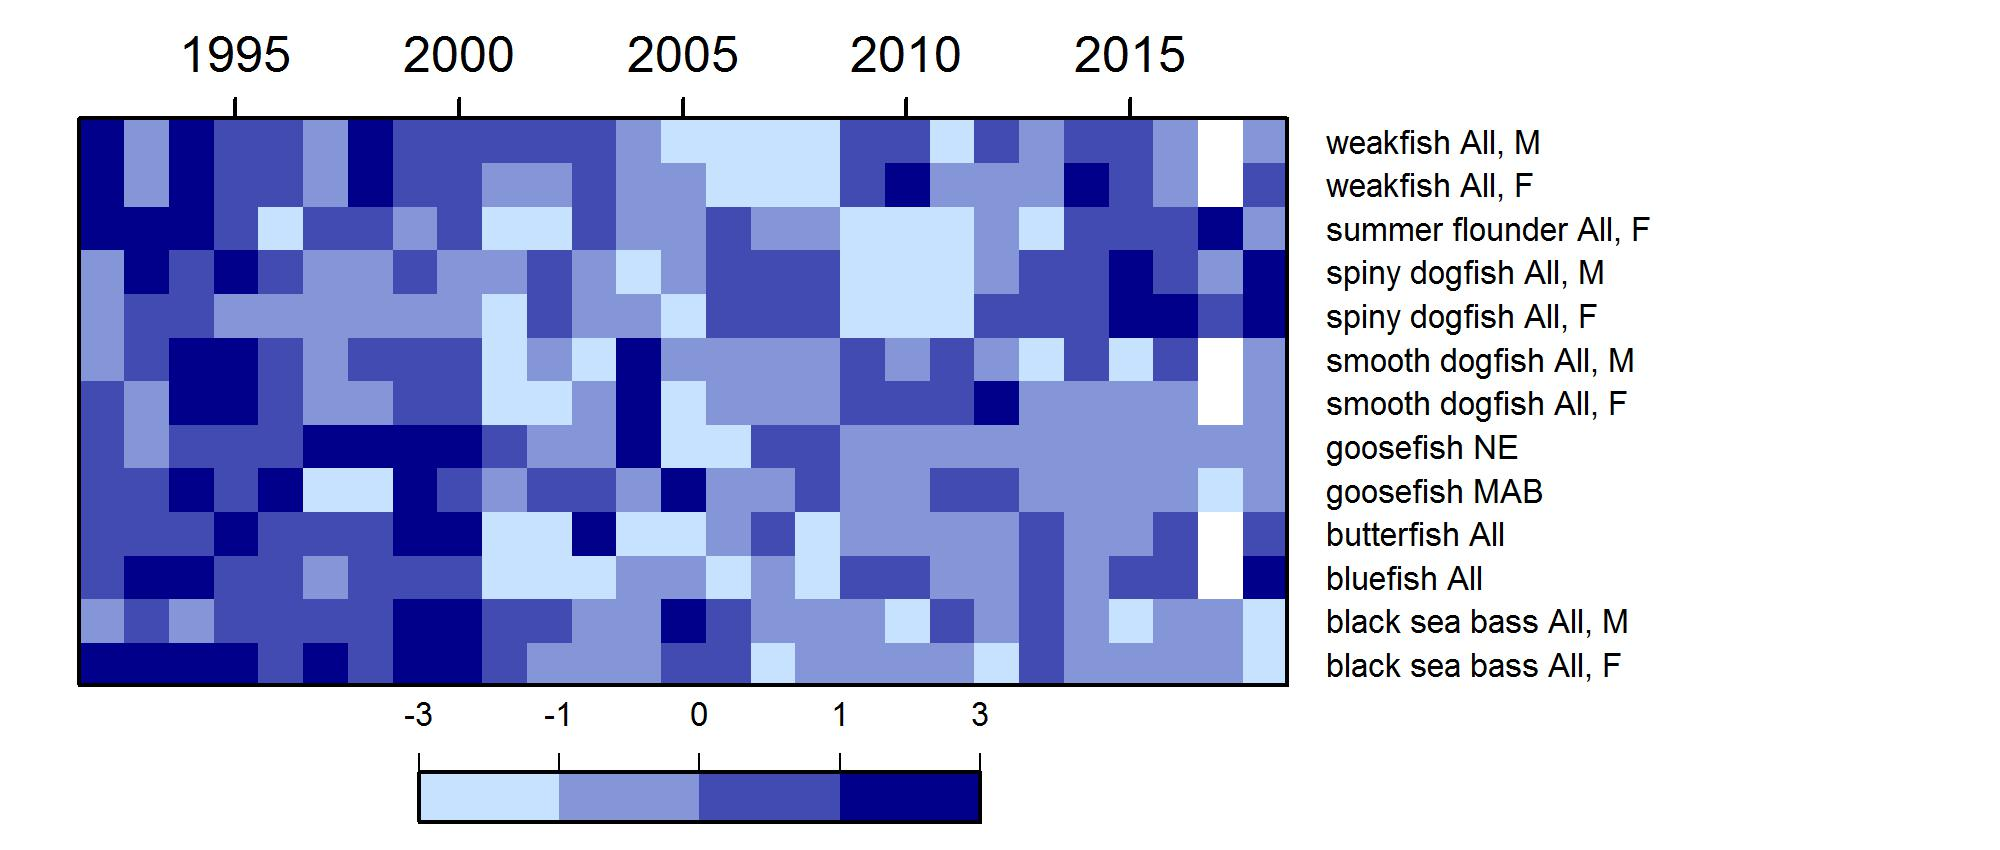
\includegraphics[width=\textwidth]{C:/Users/kimberly.bastille/Documents/GitHub/SOE-MAFMC/images/MAFMC_Fish_Condition_2019} 

}

\caption{Condition factor for MAFMC managed species.}\label{fig:mab-cf}
\end{figure}

\subsection{Fish productivity (MAB)}\label{fish-productivity-mab}

We describe patterns of aggregate fish productivity in the Mid-Atlantic
with the small fish per large fish anomaly indicator, derived from NEFSC
bottom trawl survey data (Fig. \ref{fig:MAB-recruitment}). The indicator
shows that productivity has been relatively low in this region since
2010. Recent increases in the indicator have been driven by strong
productivity years for witch flounder, silver hake, and winter flounder.

\begin{figure}

{\centering \includegraphics{SOE-MAFMC-2019_files/figure-latex/MAB-recruitment-1} 

}

\caption{Small fish per large fish biomass anomaly in the Mid-Atlantic Bight. The summed anomaly across species is shown by the black line.}\label{fig:MAB-recruitment}
\end{figure}

\subsection{Larval diversity (MAB)}\label{larval-diversity-mab}

Fluctuations in larval diversity from NEFSC ECOMON and bottom trawl
surveys reflect changing dominance of forage fish, hake, and haddock. In
fall, the decrease in diversity since 2010 is driven by high abundance
of menhaden and hake larvae. In spring, both diversity and species
richness declined to a time series low due to the dominance of sandlance
and haddock, which are common in the northern portion of the MAB (Fig.
\ref{fig:mab-larval-div}). Too few stations were sampled in spring 2014
and 2016 and in fall 2017 to detect departures from trends in the MAB.

\begin{figure}

{\centering \includegraphics{SOE-MAFMC-2019_files/figure-latex/mab-larval-div-1} 

}

\caption{Larval diversity indices from ECOMON surveys in the Mid-Atlantic.}\label{fig:mab-larval-div}
\end{figure}

Investigations are underway to evaluate changes in timing of spawning
for managed fish species. Preliminary work with flatfishes suggests that
some inshore stocks are spawning earlier as temperatures increase. There
are implications for changes in spawning timing for fish condition and
for larval survival as match or mismatch with food sources changes;
changes in timing of peak zooplankton biomass has already been observed
for some Mid-Atlantic species (next section).

\newpage

\section{Habitat Quality and Ecosystem
Productivity}\label{habitat-quality-and-ecosystem-productivity}

Productivity of harvested fish and protected species, and therefore
sustainability of fisheries, depends on adequate habitat, which
encompasses physical and chemical conditions and biological productivity
at the base of the food web. Many harvested and protected species on the
Northeast US shelf occupy several distinct habitats throughout their
life cycle, including estuaries, nearshore coastal, and offshore
environments. The indicators in this section provide information on the
changing conditions encountered by managed species in different seasons
and across habitats, which may explain observed changes in species
distribution and productivity. Ultimately, a better understanding of
these ecological drivers may permit proactive management in a changing
system.

Some habitat management interventions have proven beneficial in the
Mid-Atlantic and throughout the Northeast US Shelf. For example, the
evidence suggests that management limiting nutrient inputs has
significantly improved water quality in Chesapeake Bay. However,
temperature in coastal and offshore habitats is trending towards
unprecedented levels, accompanied by alterations in ocean circulation
patterns. Observed changes at the base of the food web, including timing
of production and plankton community composition, affect productivity of
protected and managed species in ways we do not yet fully understand.

\subsection{Estuarine habitat quality (Chesapeake
Bay)}\label{estuarine-habitat-quality-chesapeake-bay}

Many important MAFMC managed species use estuarine habitats as nurseries
or are considered estuarine and nearshore coastal-dependent (summer
flounder, scup, black sea bass, and bluefish), and interact with other
important estuarine-dependent species (e.g., striped bass and menhaden).
An integrated measure of multiple water quality criteria shows a
significantly increasing proportion of Chesapeake Bay waters meeting or
exceeding EPA water quality standards over time
({[}\protect\hyperlink{ref-zhang_chesapeake_2018}{6}{]}; Fig.
\ref{fig:cb-attainment}). This pattern was statistically linked to total
nitrogen reduction, indicating responsiveness of water quality status to
management actions implemented to reduce nutrients. Water quality trends
and status may be used to inform aquaculture siting decisions in
Chesapeake Bay.

\begin{figure}

{\centering \includegraphics{SOE-MAFMC-2019_files/figure-latex/cb-attainment-1} 

}

\caption{Estimated water quality standards attainment of Chesapeake Bay tidal waters for the combined assessment of dissolved oxygen, underwater bay grasses/water clarity and chlorophyll a using rolling three year assessment periods.}\label{fig:cb-attainment}
\end{figure}

\subsection{Ocean circulation and surface temperature
(coastwide)}\label{ocean-circulation-and-surface-temperature-coastwide}

The position of the northern edge of the Gulf Stream has been moving to
the north since the late 1950s, with an increasing rate since 2009 (Fig.
\ref{fig:GSI}). The most northerly positions ever recorded were observed
over the most recent years (2014-2017). A more northerly Gulf Stream
position is associated with warmer ocean temperature on the Northeast US
shelf {[}\protect\hyperlink{ref-zhang_role_2007}{1}{]}, a higher
proportion of Atlantic Temperate Slope Water in the Northeast Channel,
and increased sea surface height along the U.S. east coast
{[}\protect\hyperlink{ref-goddard_extreme_2015}{2}{]}.

\begin{figure}

{\centering \includegraphics{SOE-MAFMC-2019_files/figure-latex/GSI-1} 

}

\caption{Index representing changes in the location of the Gulf Stream north wall. Positive values represent a more northerly Gulf Stream position.}\label{fig:GSI}
\end{figure}

Globally, 2018 was the 4th warmest year on record and the last four
years were the warmest on record. Since the 1860's, the Northeast US
shelf sea surface temperature (SST) has exhibited an overall warming
trend, with the past decade measuring well above the long term average
(and the trendline; Fig. \ref{fig:long-term-sst}).

\begin{figure}

{\centering \includegraphics{SOE-MAFMC-2019_files/figure-latex/long-term-sst-1} 

}

\caption{Average annual sea surface temperature (SST) over the Northeast US Shelf}\label{fig:long-term-sst}
\end{figure}

\subsection{Ocean temperature, surface and bottom
(MAB)}\label{ocean-temperature-surface-and-bottom-mab}

The regional ocean is warming. Surface and bottom temperature in the MAB
averaged over all seasons has trended warmer since the early 1980s;
while seasonally temperatures have trended warmer in spring, summer, and
fall. The 2018 summer sea surface temperatures were the third highest on
record in the Mid-Atlantic, although temperatures during the other
seasons were near or slightly below average (Figs.
\ref{fig:MAB-SST-insitu}, \ref{fig:MAB-bot-temp}).

\begin{figure}

{\centering \includegraphics{SOE-MAFMC-2019_files/figure-latex/MAB-SST-insitu-1} 

}

\caption{MAB seasonal sea surface time series overlaid onto 2018 seasonal spatial anomalies.}\label{fig:MAB-SST-insitu}
\end{figure}

\begin{figure}

{\centering \includegraphics{SOE-MAFMC-2019_files/figure-latex/MAB-bot-temp-1} 

}

\caption{Annual bottom temperatures in the Mid-Atlantic Bight.}\label{fig:MAB-bot-temp}
\end{figure}

\subsection{Primary production (MAB)}\label{primary-production-mab}

Phytoplankton primary production is a function of biomass, light, and
temperature, and sets the overall level of potential fish and fishery
productivity in an ecosystem (Fig. \ref{fig:prod-potential}). There is a
trend of increasing primary production in the Mid-Atlantic, primarily
driven by increased summer production, which is due to warmer
temperatures and increased bacterial remineralization and nutrient
recycling (Fig. \ref{fig:PP-OCCI}). This increased productivity is most
likely from smaller-celled species that contribute less to fish
production compared to larger phytoplankton. The fall of 2018 had an
above average phytoplankton bloom (Fig. \ref{fig:mab-chl-weekly}), most
likely comprised of larger diatom species, with the highest
concentrations near the shelf break, which is the same region that
experienced below average temperatures in the fall (Fig.
\ref{fig:MAB-SST-insitu}).

\begin{figure}

{\centering 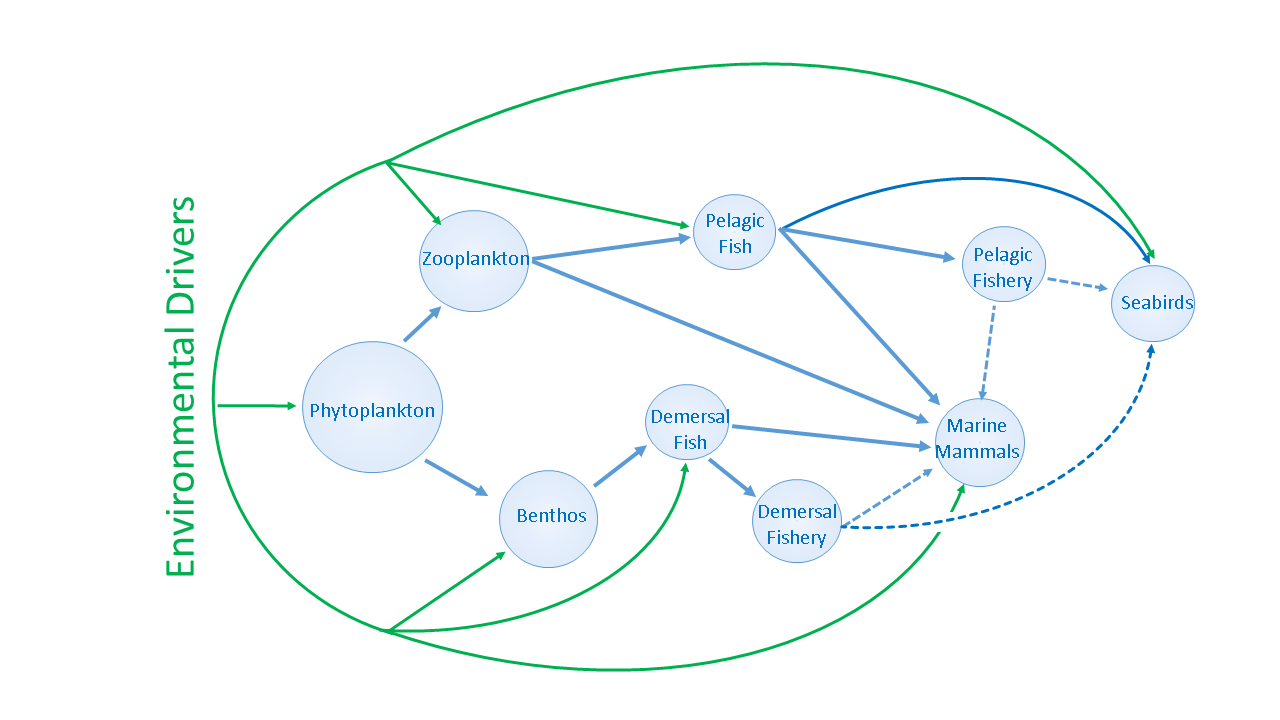
\includegraphics[width=\linewidth]{C:/Users/kimberly.bastille/Documents/GitHub/SOE-MAFMC/images/SOE_Network_Diagram} 

}

\caption{Simplified representation of the pathways linking primary production and environmental driver throughout a fishery ecosystem. The important societal benefits that derive from sustainable fisheries depend directly on a sequence of events starting at the base of the food web. The production of fish and shellfish available for harvest by the fisheries follows pathways of energy flow from phytoplankton and zooplankton to different parts of the food web. The production at each component further depends on the effect of a host of environmental drivers including temperature, salinity, and other factors.}\label{fig:prod-potential}
\end{figure}

\begin{figure}

{\centering \includegraphics{SOE-MAFMC-2019_files/figure-latex/mab-chl-weekly-1} 

}

\caption{Weekly chlorophyll concentrations in the Mid-Atlantic are shown by the colored line for 2018. The long-term mean is shown in black, and shading indicates +/- 1 sample SD.}\label{fig:mab-chl-weekly}
\end{figure}

\begin{figure}

{\centering \includegraphics{SOE-MAFMC-2019_files/figure-latex/PP-OCCI-1} 

}

\caption{Monthly primary production trends show the annual cycle (i.e. the peak during the summer months) and the changes over time for each month.}\label{fig:PP-OCCI}
\end{figure}

\subsection{Zooplankton (MAB)}\label{zooplankton-mab}

The most abundant zooplankton species in the MAB are \emph{Centropages
typicus}, \emph{Psuedocalanus} spp., and \emph{Temora longicornis}
{[}\protect\hyperlink{ref-morse_distinct_2017}{7}{]}. \emph{Calanus
finmarchicus} are also abundant in the MAB and are important prey for
larval fish and the North Atlantic right whale. Annually, there has been
a significant decrease in \emph{Pseudocalanus} and in recent years a
decreasing trend of \emph{Calanus finmarchicus} (Fig.
\ref{fig:MAB-zoo-abund}). Seasonally, \emph{Temora longicornis} have
decreased during the fall, while a decrease in fall concentration and an
increase in spring concentration of \emph{Centropages typicus} (Fig.
\ref{fig:MAB-oi-zoo}) corresponds to a shift in timing of their peak
concentration from late fall to early spring beginning in the late 1980s
{[}\protect\hyperlink{ref-bi_decadal_2014}{8}{]}.

\begin{figure}

{\centering \includegraphics{SOE-MAFMC-2019_files/figure-latex/MAB-zoo-abund-1} 

}

\caption{Abundance anomaly time series for key zooplankton species found in the MAB.}\label{fig:MAB-zoo-abund}
\end{figure}

\begin{figure}

{\centering \includegraphics{SOE-MAFMC-2019_files/figure-latex/MAB-oi-zoo-1} 

}

\caption{Seasonal abundance of key zooplankton species in the MAB.}\label{fig:MAB-oi-zoo}
\end{figure}

Changes in the abundance of the larger \emph{Calanus finmarchicus} are
also reflected in the size distribution of the copepods. The small-large
copepod index is a measure of the relative size composition of the
dominant copepod taxa. During the 1990s and early 2000s the positive
index was driven by high relative abundance of smaller bodied copepods
and a lower relative abundance of \emph{Calanus finmarchicus}. This
period was also identified with regime shifts to lower fish recruitment
{[}\protect\hyperlink{ref-perretti_regime_2017}{3}{]}. The current trend
in the index suggests an increase in the relative abundance of smaller
bodied copepods (Fig. \ref{fig:MAB-sli}).

\begin{figure}

{\centering \includegraphics{SOE-MAFMC-2019_files/figure-latex/MAB-sli-1} 

}

\caption{MAB small-large zooplankton index and the annual primary production anomaly.}\label{fig:MAB-sli}
\end{figure}

Changes in primary productivity, phytoplankton and zooplankton
composition and abundance affect the food web and may be related to
observed changes in fish condition, recruitment patterns, and forage
fish energy content. However, more research and analyses are needed to
directly link these connections. Any attempt to predict how the
ecosystem will respond to changes in climate and fishing patterns
ultimately will depend on understanding these connections. Our objective
is to shed light on these fundamental issues and to document changes
affecting human communities and the fishery ecosystem on which we
depend.

\section{Contributors}\label{contributors}

\textbf{Editors} (NOAA NMFS Northeast Fisheries Science Center, NEFSC):
Sarah Gaichas, Sean Hardison, Scott Large, Sean Lucey

\textbf{Contributors} (NEFSC unless otherwise noted): Lisa Calvo
(Rutgers), Patricia Clay, Lisa Colburn, Geret DePiper, Michael Fogarty,
Paula Fratantoni, Kevin Friedland, Sarah Gaichas, James Gartland
(Virginia Institute of Marine Science), Heather Haas, Sean Hardison,
Kimberly Hyde, Terry Joyce (Woods Hole Oceanographic Institute), John
Kosik, Steve Kress and Don Lyons (National Audubon Society's Seabird
Restoration Program), Sean Lucey, Chris Melrose, Ryan Morse, Kimberly
Murray, Chris Orphanides, Richard Pace, Charles Perretti, Karl Roscher
(Maryland Department of Natural Resources), Vincent Saba, Laurel Smith,
Mark Terceiro, John Walden, Harvey Walsh, Mark Wuenschel, and Qian Zhang
(Unversity of Maryland and US EPA Chesapeake Bay Program).

\newpage 

\section{Document Orientation}\label{document-orientation}

The figure format is illustrated in Fig \ref{fig:docformat}a. Trend
lines are shown when slope is significantly different from 0 at the p
\textless{} 0.05 level. An orange line signifies an overall positive
trend, and purple signifies a negative trend. To minimize bias
introduced by small sample size, no trend is fit for \textless{} 30 year
time series. Dashed lines represent mean values of time series unless
the indicator is an anomaly, in which case the dashed line is equal to
0. Shaded regions indicate the past ten years. If there are no new data
for 2018, the shaded region will still cover this time period. The
spatial scale of indicators is either coastwide, Mid-Atlantic states
(New York, New Jersey, Delaware, Maryland, Virginia, North Carolina), or
at the Mid-Atlantic Bight (MAB) Ecosystem Production Unit (EPU, Fig.
\ref{fig:docformat}b) level.

\begin{figure}

{\centering \includegraphics{SOE-MAFMC-2019_files/figure-latex/docformat-1} 

}

\caption{Document orientation. a. Key to figures. b.The Northeast Large Marine Ecosystem.}\label{fig:docformat}
\end{figure}

Fish and invertebrates are aggregated into similar feeding categories
(Table \ref{tab:species-groupings}) to evaluate ecosystem level trends
in predators and prey.

\begin{table}[!h]

\caption{\label{tab:species-groupings}Feeding guilds and management bodies.}
\centering
\resizebox{\linewidth}{!}{
\fontsize{10}{12}\selectfont
\begin{tabular}{>{\raggedright\arraybackslash}p{2cm}>{\raggedright\arraybackslash}p{4cm}>{\raggedright\arraybackslash}p{2cm}>{\raggedright\arraybackslash}p{5cm}>{\raggedright\arraybackslash}p{6cm}}
\toprule
\textbf{Guild} & \textbf{MAFMC} & \textbf{Joint} & \textbf{NEFMC} & \textbf{State or Other}\\
\midrule
Apex Predator & NA & NA & NA & bluefin tuna, shark uncl, swordfish, yellowfin tuna\\
\cmidrule{1-5}
Piscivore & bluefish, summer flounder & goosefish, spiny dogfish & acadian redfish, atlantic cod, atlantic halibut, clearnose skate, little skate, offshore hake, pollock, red hake, silver hake, smooth skate, thorny skate, white hake, winter skate & fourspot flounder, john dory, sea raven, striped bass, weakfish, windowpane\\
\cmidrule{1-5}
Planktivore & atlantic mackerel, butterfish, longfin squid, northern shortfin squid & NA & atlantic herring & alewife, american shad, blackbelly rosefish, blueback herring, cusk, longhorn sculpin, lumpfish, menhaden, northern sand lance, northern searobin, sculpin uncl\\
\cmidrule{1-5}
Benthivore & black sea bass, scup, tilefish & NA & american plaice, barndoor skate, crab,red deepsea, haddock, ocean pout, rosette skate, winter flounder, witch flounder, yellowtail flounder & american lobster, atlantic wolffish, blue crab, cancer crab uncl, chain dogfish, cunner, jonah crab, lady crab, smooth dogfish, spider crab uncl, squid cuttlefish and octopod uncl, striped searobin, tautog\\
\cmidrule{1-5}
Benthos & atlantic surfclam, ocean quahog & NA & sea scallop & blue mussel, channeled whelk, sea cucumber, sea urchin and sand dollar uncl, sea urchins, snails(conchs)\\
\bottomrule
\end{tabular}}
\end{table}

\newpage 

\section*{References}\label{references}
\addcontentsline{toc}{section}{References}

\hypertarget{refs}{}
\hypertarget{ref-zhang_role_2007}{}
1. Zhang R, Vallis GK. The role of bottom vortex stretching on the path
of the North Atlantic western boundary current and on the northern
recirculation gyre. Journal of Physical Oceanography. 2007;37:
2053--2080.
doi:\href{https://doi.org/10.1175/JPO3102.1}{10.1175/JPO3102.1}

\hypertarget{ref-goddard_extreme_2015}{}
2. Goddard PB, Yin J, Griffies SM, Zhang S. An extreme event of
sea-level rise along the Northeast coast of North America in 2009--2010.
Nature Communications. 2015;6.
doi:\href{https://doi.org/10.1038/ncomms7346}{10.1038/ncomms7346}

\hypertarget{ref-perretti_regime_2017}{}
3. Perretti C, Fogarty M, Friedland K, Hare J, Lucey S, McBride R, et
al. Regime shifts in fish recruitment on the Northeast US Continental
Shelf. Marine Ecology Progress Series. 2017;574: 1--11.
doi:\href{https://doi.org/10.3354/meps12183}{10.3354/meps12183}

\hypertarget{ref-greene_remote_2013}{}
4. Greene CH, Meyer-Gutbrod E, Monger BC, McGarry LP, Pershing AJ,
Belkin IM, et al. Remote climate forcing of decadal-scale regime shifts
in Northwest Atlantic shelf ecosystems. Limnology and Oceanography.
2013;58: 803--816.
doi:\href{https://doi.org/10.4319/lo.2013.58.3.0803}{10.4319/lo.2013.58.3.0803}

\hypertarget{ref-pace_statespace_2017}{}
5. Pace RM, Corkeron PJ, Kraus SD. State--space mark--recapture
estimates reveal a recent decline in abundance of North Atlantic right
whales. Ecology and Evolution. 2017;7: 8730--8741.
doi:\href{https://doi.org/10.1002/ece3.3406}{10.1002/ece3.3406}

\hypertarget{ref-zhang_chesapeake_2018}{}
6. Zhang Q, Murphy RR, Tian R, Forsyth MK, Trentacoste EM, Keisman J, et
al. Chesapeake Bay's water quality condition has been recovering:
Insights from a multimetric indicator assessment of thirty years of
tidal monitoring data. Science of the Total Environment. 2018;637-638:
1617--1625.
doi:\href{https://doi.org/10.1016/j.scitotenv.2018.05.025}{10.1016/j.scitotenv.2018.05.025}

\hypertarget{ref-morse_distinct_2017}{}
7. Morse R, Friedland K, Tommasi D, Stock C, Nye J. Distinct zooplankton
regime shift patterns across ecoregions of the U.S. Northeast
continental shelf Large Marine Ecosystem. Journal of Marine Systems.
2017;165: 77--91.
doi:\href{https://doi.org/10.1016/j.jmarsys.2016.09.011}{10.1016/j.jmarsys.2016.09.011}

\hypertarget{ref-bi_decadal_2014}{}
8. Bi H, Ji R, Liu H, Jo Y-H, Hare JA. Decadal Changes in Zooplankton of
the Northeast U.S. Continental Shelf. PLOS ONE. 2014;9: e87720.
doi:\href{https://doi.org/10.1371/journal.pone.0087720}{10.1371/journal.pone.0087720}


\end{document}
